\documentclass[12pt,a4paper]{article}
\usepackage[utf8]{inputenc}

% Bibliography management
\usepackage[
backend=biber,
citestyle=authoryear,
style=alphabetic,
sorting=ynt
]{biblatex}
\addbibresource{bibliography.bib}
% \usepackage[nottoc]{tocbibind}

% Code Listings
\usepackage{listings}
\usepackage{listings-golang} % import this package after listings
\usepackage{color}

% Images
% \usepackage{graphicx}
% \graphicspath{ {images/} }

% Diagrams
\usepackage{tikz}
\usetikzlibrary{shapes, arrows, arrows.meta}

\setlength{\abovecaptionskip}{5px}

\title{A compositional toolkit for the construction of concurrent Web servers}
\author{Michal Bock}
\date{}

\lstset{ % add your own preferences
    frame=single,
    basicstyle=\footnotesize,
    keywordstyle=\color{blue},
    numbers=none,
    showstringspaces=false, 
    stringstyle=\color{red},
    tabsize=4,
    language=Golang,
    belowskip=0px
}

% Define block styles
\tikzstyle{listener} = [rectangle, draw, fill=gray!60, 
    text width=5em, text centered, minimum height=4em]
\tikzstyle{component} = [rectangle, draw, fill=white, 
    text width=7em, text centered, minimum height=4em]
\tikzstyle{writer} = [rectangle, draw, fill=gray!30, 
    text width=5em, text centered, minimum height=4em]
\tikzstyle{line} = [draw, -latex']

\usepackage[parfill]{parskip}
\usepackage[labelfont=bf]{caption}

\begin{document}

%%%%%%%%%%%%%%%%%%%%%%%%%%%%% Title page %%%%%%%%%%%%%%%%%%%%%%%%%%%%%%
\maketitle
\thispagestyle{empty}

%%%%%%%%%%%%%%%%%%%%%%%%%%%%% Abstract %%%%%%%%%%%%%%%%%%%%%%%%%%%%%%%%

\newpage
\section*{Abstract}
\begin{quote}
The goal of this project is to construct a well-structured
library of communicating components, in the Go language, to support
the programming of a family of webservers that could range in scale 
from a full-scale commercial server to an embedded server used to provide 
a browser-based GUI to a specific application.
\end{quote}

%%%%%%%%%%%%%%%%%%%%%%%%%%%%% Contents %%%%%%%%%%%%%%%%%%%%%%%%%%%%%%%%
\newpage
\pagenumbering{arabic}
\tableofcontents

%%%%%%%%%%%%%%%%%%%%%%%%%%%%% Introduction %%%%%%%%%%%%%%%%%%%%%%%%%%%%
\newpage
\section{Introduction}
In this section I first introduce the motivation behind this project
and an overview of the used design. Then I follow
by explaining the basics of message passing concurrency and the basics
of the go programming language, which was used to implement the proposed 
toolkit. I finish by reviewing related work done on similar problems.

\subsection{Motivation}
The vast majority of web server frameworks such as Apache
use a single handler function that
computes responses to all types of client requests. When a request comes in a 
worker is allocated from a pool of workers and it then executes the handler function
and returns the result to the client.

This project examines an alternative approach for building web-servers. 
I propose to construct a web-server as a network of highly specialized 
communicating components. The communication should be done using
message passing. This builds on the premise that we can deal
with different types of requests using different single purpose components.

The main advantages of the proposed architecture are that it is easy to understand
and configure. A conceptual design of response generation from a request translates 
directly into a server architecture. That is a flow chart representing a transition
of a request into a response can be directly translated into program code.
Due to the compositional nature of this design its also very easy to reuse code
and use wrappers to introduce new behaviors such as caching of responses.

\subsection{Proposed Architecture}
The overall server architecture can be explained as follows.
The components each representing a single action are plugged together into 
a pipeline using channels to implement complex behaviors. The incoming
request together with the result computed so far and other 
information needed for computation and writing the result back to the client
are passed through the channels.

The incoming request are fed into the input end of the pipeline and 
after passing through the whole network the response is written to the
client on the other end. Hence, we can view this server
as a pipeline that transfers requests into responses.

To implement this architecture I have constructed a toolkit called 
\texttt{mpserver}, that allows the construction of such web-servers.
It uses default \texttt{http} package to handle the details of
the HTTP protocol. The toolkit itself concentrates on structuring the 
web-server.


\subsection{Introduction to Message passing Concurrency}
This section first introduces channels and then presents the Message
Passing Concurrency Paradigm.

\subsubsection{Channels}
Channel is a FIFO queue of pending messages. It can be accessed by two
primitive operations, which are send and receive. To start communication
a process sends a value to the channel. Another process acquires the message
by receiving from the channel. Sending a message can be asynchronous (nonblocking)
or synchronous (blocking). Note that receiving message is invariably blocking.
\cite[293]{book:foundations}

\subsubsection{Message Passing Concurrency}
Message Passing Concurrency is a style of Concurrent Programming, in which
processes communicate using channels and communication is the only way
any two processes can synchronize. Hence, this style does not 
suffer any problems that arise from using shared memory for communication 
and synchronization by multiple concurrent processes.


\subsection{Introduction to go}
Go is a C like programming language. Its main advantage is 
that it has a lot of concurrent constructs built natively into it.
This is also the reason why it was chosen as implementation language 
for this project.
In this section I introduce the main concurrency constructs that are
present in the language and its type system. Other features
of the language are explained, when they are used.

\subsubsection{Goroutines}
A goroutine is a lightweight thread managed by the Go runtime \cite{Tour}.

\subsubsection{Channels}
\subsubsection{Objects methods and Interfaces}


\subsection{Related work}
% TODO: maybe move to a later section
Similar work has been examined by James Whitehead II in \cite{whitehead}.
However, his approach is rather different than the approach used 
in this project. He uses reader-writer pairs for communication between
two different components in the network. This requires to construct the
reader and writer objects for each pair of communicating components
for all requests.
In order to construct these readers and writers a connection object is 
passed through the network.
I believe this indirect approach introduces unnecessary overhead and 
makes it more difficult to understand how the toolkit works.

However, the readers-writers model has one significant advantage over
my proposed model. This advantage is the ability to
perform computation in different components at the same time. This is
is not possible using my message passing approach, as firstly a 
component needs to finish its work and afterwards send the result to the next
component, which can only then start working.
However, the readers-writers behavior can be mimicked by my implementation 
if required.

\subsection{Report overview}
In Chapter \ref{sec:arch} I analyze design of a few simple server examples 
in the suggested framework. Chapter \ref{sec:impl} describes my implementation
of the proposed toolkit. Then in Chapter \ref{sec:examples} I present
implementations in my framework of servers described in chapter \ref{sec:arch}.

In chapter \ref{sec:test} I present results of performance tests of equivalent 
servers implemented in my framework, in pure go, in toolkit described
in \cite{whitehead} and using Apache framework. Finally in chapter 
\ref{sec:conclusion} I summarize the results and achievements of this 
project and present ideas for future work.

%%%%%%%%%%%%%%%%%%%%%%%%%%%%%%%%%%%%%%%%%%%%%%%%%%%%%%%%%%%%%%%%%%%%%%%
%%%%%%%%%%%%%%%%%%%%%%%%%%%%% Architecture %%%%%%%%%%%%%%%%%%%%%%%%%%%%
%%%%%%%%%%%%%%%%%%%%%%%%%%%%%%%%%%%%%%%%%%%%%%%%%%%%%%%%%%%%%%%%%%%%%%%

\newpage
\section{Architecture}
\label{sec:arch}
The most appealing thing about the proposed compositional architecture is that
it makes implementing the server very easy. If you can construct a flow chart 
representing the conversion of a request into a response, then this flow chart
can be directly translated into a program.

In this section I introduce a few example web-servers and their conceptual
design using the proposed architecture. I also introduce a wrapper 
solution used for caching and load balancing.
Finally I compare these designs to the set up of equivalent Apache servers.

\subsection{Hello World!}
\label{sec:helloWorld}
The simplest example is a Hello world! server. This server replies with a 
Hello world! message to all requests and can be represented by the diagram
in Figure \ref{fig:helloWorld}.

\begin{figure}[h]
\centering
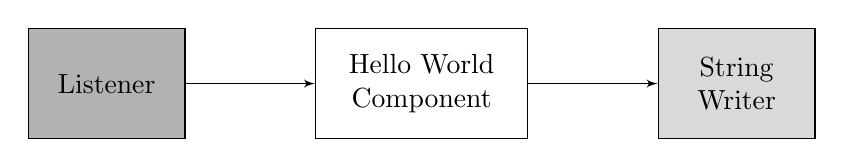
\begin{tikzpicture}[node distance = 2cm, auto]
    % Nodes
    \node [listener] (listener) {Listener};
    \node [component, right of=listener, node distance=4cm] (hello) {Hello World Component};
    \node [writer, right of=hello, node distance=4cm] (writer) {String Writer};
    % Edges
    \path [line] (listener) -- (hello);
    \path [line] (hello) -- (writer);
\end{tikzpicture}
\caption[scale=1.0]{Hello world! server architecture.}
\label{fig:helloWorld}
\end{figure}

The \texttt{Listener} represents the 
part of the program that gets requests and feeds them to the network.
The \texttt{Hello World Component} returns the Hello World! string as a result 
for the request and the \texttt{String Writer} writes the text response 
back to the client.

This is a good example of the basic components of the suggested framework.
We can call the three main parts the Listener, Processor and Writer, where
the Listener catches the incoming requests and feeds them into the network,
the Processor processes them and the writer writes the generated result 
back to the client.

\subsection{File Server}
Architecture of a simple file server follows the architecture of the Hello world!
server introduced above. It consists of a \texttt{Listener}, which catches the requests,
\texttt{File Getter}, what is a function that gets the requested file (that is it loads it or 
constructs its absolute path) and finally there is a \texttt{File Writer}, which
writes the file to the client. The architecture is shown in Figure \ref{fig:fileServer}.
\\
\begin{figure}[h]
\centering
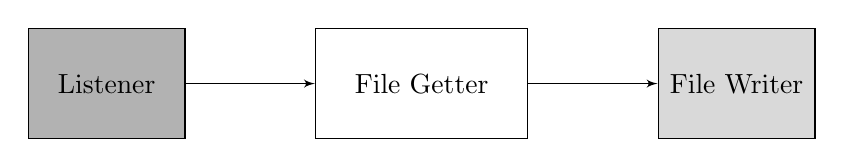
\begin{tikzpicture}[node distance = 2cm, auto]
    % Nodes
    \node [listener] (listener) {Listener};
    \node [component, right of=listener, node distance=4cm] (getter) {File Getter};
    \node [writer, right of=getter, node distance=4cm] (writer) {File Writer};
    % Edges
    \path [line] (listener) -- (getter);
    \path [line] (getter) -- (writer);
\end{tikzpicture}
\caption[scale=1.0]{File server.}
\label{fig:fileServer}
\end{figure}

If we want to compress some subset of files, we can just add a \texttt{Splitter}
that sends files that are supposed to be compressed to a \texttt{Gzip Writer}, which
compresses the file and writes the result to the client. The rest of the files
will be passed to the standard \texttt{File Writer}. This architecture is shown in
Figure \ref{fig:fileServer2}.

\begin{figure}[h]
\centering
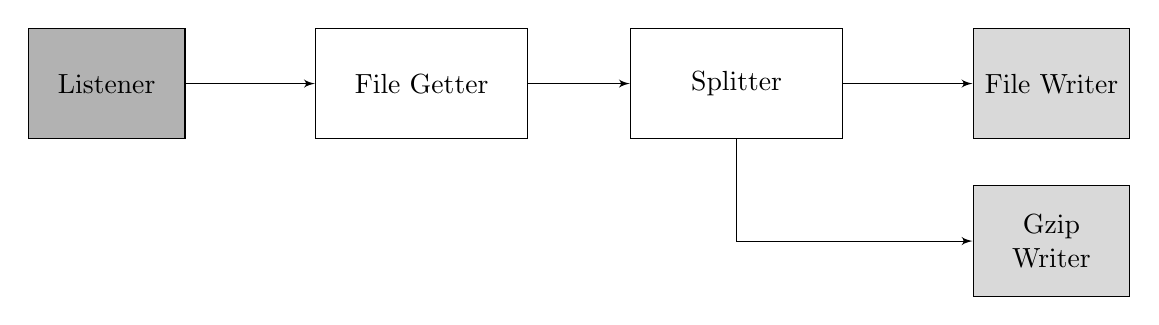
\begin{tikzpicture}[node distance = 2cm, auto]
    % Nodes
    \node [listener] (listener) {Listener};
    \node [component, right of=listener, node distance=4cm] (getter) {File Getter};
    \node [component, right of=getter, node distance=4cm] (splitter) {Splitter};
    \node [writer, right of=splitter, node distance=4cm] (fwriter) {File Writer};
    \node [writer, below of=fwriter] (gwriter) {Gzip Writer};
    % Edges
    \path [line] (listener) -- (getter);
    \path [line] (getter) -- (splitter);
    \path [line] (splitter) -- (fwriter);
    \path [line] (splitter) |- (gwriter);
\end{tikzpicture}
\caption[scale=1.0]{File server with compression.}
\label{fig:fileServer2}
\end{figure}

\subsection{Caching}
Suppose we have a worker component, which performs some expensive computation
and hence we want to cache its output.
Using the proposed architecture we can just wrap the worker in a caching layer.
That is we only run the worker component if we don't have the result
in the cache, otherwise we just return the stored result. 
This design is show in Figure \ref{fig:caching}.

\begin{figure}[h]
\centering
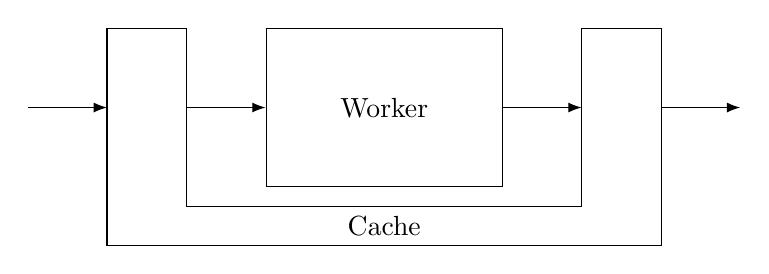
\begin{tikzpicture}[
    workerWidth/.style={minimum width=3cm},
    workerHeight/.style={minimum height=2cm},
    UWidth/.style={minimum width=1cm},
    every node/.style={
        text centered,
        }
        ]
    \node[workerWidth, workerHeight, draw] (worker) at (0, 0) {Worker};

    \node[anchor=north, workerWidth, yshift=-0.25cm] (cache) at (worker.south) {Cache};

    \node[anchor=east, workerHeight, UWidth, xshift=-1cm] (left) at (worker.west) {};
    \node[anchor=west, workerHeight, UWidth, xshift=1cm] (right) at (worker.east) {};

    \draw (left.north west) -- (left.west |- cache.south) -- (right.east |- cache.south) -- (right.north east) -- (right.north west) -- (right.west |- cache.north) -- (left.east |- cache.north) -- (left.north east) -- cycle;

    \draw[<-, >={Latex}] (left.west) -- ++(-1, 0);
    \draw[->, >={Latex}] (left.east) -- (worker.west);
    \draw[->, >={Latex}] (worker.east) -- (right.west);
    \draw[->, >={Latex}] (right.east) -- ++(1, 0);
\end{tikzpicture}\caption[scale=1.0]{Caching output of a worker component.}
\label{fig:caching}
\end{figure}

\subsection{Load Balancing}
If there is a lot of traffic in a certain part of the network we can
increase the throughput there
by creating multiple instances of the components in this part of 
the pipeline. The incoming request will then be passed to the component that is 
ready first. When the load in a given part of the pipeline decreases,
we can shut down the created components.

The benefit of the proposed architecture is that, we can do these adjustments
in runtime.
That is, based on current number of requests going through a certain part of 
the network we can decide to add or remove parts of the pipeline. This does not
have to be only adding components locally.
If we use channels over network then
we can connect to other servers and distribute the workload among them.
Hence we can start or shut down other servers based on the current traffic.
    Figure \ref{fig:loadBalancing}.

\begin{figure}[h]
\centering
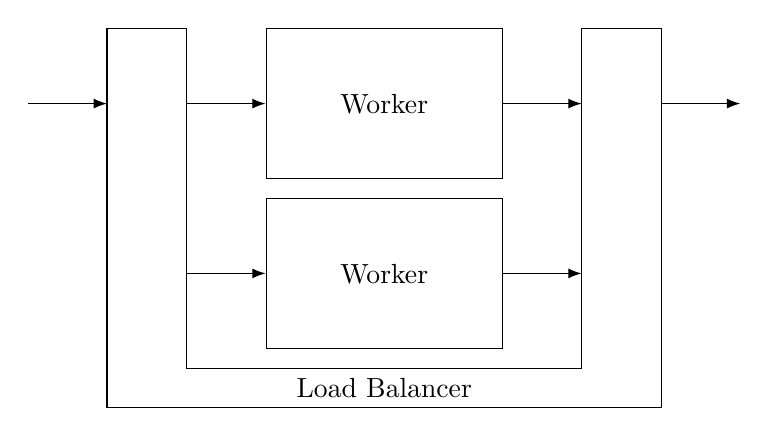
\begin{tikzpicture}[
    workerWidth/.style={minimum width=3cm},
    workerHeight/.style={minimum height=1.9cm},
    UWidth/.style={minimum width=1cm},
    every node/.style={
        text centered,
        }
        ]
    \node[workerWidth, workerHeight, draw] (worker) at (0, 0) {Worker};
    \node[workerWidth, workerHeight, yshift=-1.2cm, draw] (worker2) at (worker.south) {Worker};

    \node[anchor=north, workerWidth, yshift=-0.25cm] (cache) at (worker2.south) {Load Balancer};

    \node[anchor=east, workerHeight, UWidth, xshift=-1cm] (left) at (worker.west) {};
    \node[anchor=west, workerHeight, UWidth, xshift=1cm] (right) at (worker.east) {};
    \node[anchor=east, workerHeight, UWidth, xshift=-1cm] (left2) at (worker2.west) {};
    \node[anchor=west, workerHeight, UWidth, xshift=1cm] (right2) at (worker2.east) {};

    \draw (left.north west) -- (left.west |- cache.south) -- (right.east |- cache.south) -- (right.north east) -- (right.north west) -- (right.west |- cache.north) -- (left.east |- cache.north) -- (left.north east) -- cycle;

    \draw[<-, >={Latex}] (left.west) -- ++(-1, 0);
    \draw[->, >={Latex}] (left.east) -- (worker.west);
    \draw[->, >={Latex}] (worker.east) -- (right.west);
    \draw[->, >={Latex}] (left2.east) -- (worker2.west);
    \draw[->, >={Latex}] (worker2.east) -- (right2.west);
    \draw[->, >={Latex}] (right.east) -- ++(1, 0);
\end{tikzpicture}\caption[scale=1.0]{
    Managing load in a given part of the network.
    One of the workers can be shut down or more workers can be added.
}
\label{fig:loadBalancing}
\end{figure}

\subsection{Comparison to Apache server configuration}

\subsection{Summary}

%%%%%%%%%%%%%%%%%%%%%%%%%%%%%%%%%%%%%%%%%%%%%%%%%%%%%%%%%%%%%%%%%%%%%%%
%%%%%%%%%%%%%%%%%%%%%%%%%% Implementation %%%%%%%%%%%%%%%%%%%%%%%%%%%%%
%%%%%%%%%%%%%%%%%%%%%%%%%%%%%%%%%%%%%%%%%%%%%%%%%%%%%%%%%%%%%%%%%%%%%%%

\newpage
\section{Implementation}
\label{sec:impl}
In this chapter I present the implementation of my \texttt{mpserver} toolkit.
It is implemented as a go package. I start by

The web-server consists of a multiple Components which are plugged 
together using channels to form a pipeline that transforms requests 
to responses.

\subsection{Values}
\texttt{Value} is a struct type that represents the type of messages that are
passed between the components of the network. It is defined as follows:

\begin{figure}[h]
\centering
\begin{lstlisting}
type Value struct {
    Request *http.Request
    Writer http.ResponseWriter
    Result Any
    Done chan<- bool
    ResponseCode int
}
\end{lstlisting}
\caption[scale=1.0]{Declaration of type Value.}
\label{fig:Value}
\end{figure}

Here:
\begin{itemize}
  \item \texttt{Request} is the HTTP request made by the client implemented
        in the default HTTP library.

  \item \texttt{Writer} is an object that writes the response back to the client.
        Its type is \texttt{ResponseWriter}, which is implemented in the default HTTP
        package. This together with the \texttt{Request} field is set just before
        the value is fed into the network.
        This should only be used by \texttt{Writer} objects that are introduced later.


  \item \texttt{Result} is the result computed so far (initially nil). This is
        of type \texttt{Any} which is defined to be the empty interface.
        This allows values of any type to be stored there.

  \item \texttt{Done} is a signaling channel. Signal should be send on this channel,
		after the response is written at the end of the pipeline. This
        allows the connection to the client to be closed after the result
        is written.

  \item \texttt{ResponseCode} is the HTTP response code that should be 
        returned to the client. The default value of this field is 200,
        which represents a successful request.
\end{itemize}


\subsection{Components}
Component is a generic part of the pipeline with an input and output channel.
It processes the values provided on input channel and outputs the results
on the output channel. The type \texttt{Component} is defined as follows:


\begin{figure}[h]
\centering
\begin{lstlisting}
type Component func (in <-chan Value, out chan<- Value)
\end{lstlisting}
\caption[scale=1.0]{Declaration of type Component.}
\label{fig:Component}
\end{figure}

Every Component should satisfy the following:
\begin{itemize}
    \item When run Component should read values from the input channel
		  and output processed values on the output channel while the input 
		  channel is open.

    \item Component terminates normally only if its input channel is closed.

    \item Before terminating, every Component closes its output channel.

    \item Component can only close its output channel and it can only do so
    	  after its input channel have been closed.

    \item For every value that a Component reads from the input channel, 
		  it should write a value to the output channel. So, that every request 
		  gets a response.
  
\end{itemize}

\subsubsection{Making Components}
To simplify the construction of components, so that they adhere to 
the above specification the package provides a helper function that 
constructs a component using a function that maps a \texttt{Value} object 
into another \texttt{Value} object. This represents the mapping of the
input values to the output values.
The signature of this component generator is below:

\begin{figure}[h]
\centering
\begin{lstlisting}
func MakeComponent(f ComponetFunc) Component
\end{lstlisting}
\caption[scale=1.0]{Declaration of MakeComponent function.}
\label{fig:MakeComponent}
\end{figure}

Here the Component Function is a helper type with the following definition:

\begin{figure}[h]
\centering
\begin{lstlisting}
type ComponetFunc func (val Value) Value
\end{lstlisting}
\caption[scale=1.0]{Declaration of type ComponentFunc.}
\label{fig:ComponentFunc}
\end{figure}

The Component constructed by MakeComponent function reads value from the
input channel, runs provided function f on this value and then outputs the
result of f.

\subsubsection{Constant Component}
Constant Component is a simple component generator that takes a value c
of any type and returns a component that writes c to the Result field of 
all inputted values and then outputs them. It's signature is below.

\begin{figure}[h]
\centering
\begin{lstlisting}
func ConstantComponent(c Any) Component
\end{lstlisting}
\caption[scale=1.0]{Declaration of Constant Component generator.}
\label{fig:ConstantComponent}
\end{figure}


\subsection{Linking components}
The library provides a component generator Link Components that takes 
any number of components and returns a component that behaves as their 
linear combination. That is as a pipeline constructed from these components 
in the order in which they are provided. Its signature is below:

\begin{figure}[h]
\centering
\begin{lstlisting}
func LinkComponents(components ...Component) Component
\end{lstlisting}
\caption[scale=1.0]{Declaration of LinkComponents function.}
\label{fig:LinkComponents}
\end{figure}

The subcomponents are linked and run when the combined component is run. 
The last of the provided components is run in the goroutine in which
the combined component was run.

\subsection{Writers}
Writer is the end of the pipeline which writes results to the client.
The type \texttt{Writer} is defined as follows:

\begin{figure}[h]
\centering
\begin{lstlisting}
type Writer func (in <-chan Value, errChan chan<- Value)
\end{lstlisting}
\caption[scale=1.0]{Declaration of type Writer.}
\label{fig:Writer}
\end{figure}

It is a function with an input channel and a channel for reporting errors.
\begin{itemize}
	\item When a Writer writes the result to the client, it should send a signal
		  on done channel, so that the connection to the client can be closed.
	\item The writer terminates when its input channel is closed. It shouldn't
		  close the error channel, as other processes might be using it.
\end{itemize}

\subsubsection{Error Writer}
Error Writer is a function that writes error responses to the client.
It has the following signature:

\begin{figure}[h]
\centering
\begin{lstlisting}
func ErrorWriter(in <-chan Value)
\end{lstlisting}
\caption[scale=1.0]{Declaration of ErrorWriter function.}
\label{fig:ErrorWriter}
\end{figure}

It has only one input channel. The writer terminates when the channel
is closed. The channel should be closed only after all Writers that 
are using it terminated.

\subsection{Conditions and Splitter}
\subsubsection{Conditions}
Condition type is defined as follows:

\begin{figure}[h]
\centering
\begin{lstlisting}
type Condition func (val Value) bool
\end{lstlisting}
\caption[scale=1.0]{Declaration of type Condition.}
\label{fig:Condition}
\end{figure}

It is a function that takes a value and returns a boolean.

\subsubsection{Splitter}
Conditions are used in Splitter, which is a component with the 
following signature:

\begin{figure}[h]
\centering
\begin{lstlisting}
func Splitter(in <-chan Value, defOut chan<- Value, 
			  outs []chan<- Value, conds []Condition)
\end{lstlisting}
\caption[scale=1.0]{Declaration of type Splitter.}
\label{fig:Splitter}
\end{figure}

It takes an input channel, default output channel, array of output channels and array of conditions.
The number of output channels and the number of conditions should be the same.
For every input value the Splitter evaluates the conditions from first to last.
When a condition returns true the value is written to a corresponding output channel 
and the processing of the current value terminates. If all conditions return false
then the value is written to the default output channel.

\subsection{States and Session Management Component}
\subsubsection{States}
State is an interface defined as follows:

\begin{figure}[h]
\centering
\begin{lstlisting}
type State interface {
    Next(val Value) (State, error)
    Terminal() bool
    Result() Any
}
\end{lstlisting}
\caption[scale=1.0]{Declaration of interface State.}
\label{fig:State}
\end{figure}

\begin{itemize}
	\item The \texttt{Next} function returns the next state when provided with a value.
	\item The \texttt{Terminal} function indicates whether the current state is a terminal state.
	\item The \texttt{Result} function returns the result that possibly after further 
		  processing should be returned to the client.
\end{itemize}

\subsubsection{Session Management Component}
\texttt{Session Management Component} is a following component generator.

\begin{figure}[h]
\centering
\begin{lstlisting}
func SessionManagementComponent(
		initial State, seshExp time.Duration) Component
\end{lstlisting}
\caption[scale=1.0]{Declaration of Session Management Component generator.}
\label{fig:seshComp}
\end{figure}

It takes an initial state for each session and a session expiration time and 
returns a Component that behaves as a session manager. 

The component behaves as follows:

The component stores a mapping from session ids to current state of the session.

Every new request gets assigned a unique session id. Then a mapping from the generated 
id to the current state, which is generated from the initial state using the provided value,
is stored. The result of the call to the \texttt{Result} function on the next state with the provided 
value is then sent down the pipeline.

When a request with set `Session-Id` header comes in, the component gets the current 
state for the session and gets the next state for it based on the provided value.
The mapping is then updated with the generated state and the result from the current state
is passed down the pipeline.

When a session reaches a Terminal state, the session id is removed from the map
and the final result is outputted.

The states in the mapping are timestamped and are removed from the map after
the session expiration time, if they haven't finished before that.

The abstraction using states allows the users of the package to implement the
logic for the session, independently of the session management part.

\subsection{Caching}
\texttt{Cache Component} is a Component generator with the following signature:

\begin{figure}[h]
\centering
\begin{lstlisting}
func CacheComponent(worker Component, 
					expiration time.Duration) Component
\end{lstlisting}
\caption[scale=1.0]{Declaration of Cache Component generator.}
\label{fig:cacheComp}
\end{figure}

The returned component behaves as follows:
\begin{itemize}
	\item When a value is inputted that the component hasn't seen before, then
				the value is passed to the provided worker and the result is stored in
				a map.
	\item When the component gets a previously seen value, it returns the value
			  stored in the map, if it hasn't expired yet. If it expired, then the component
				treats it as a new value.
	\item Expired values are regularly deleted from the map.
\end{itemize}

For the generated component to function properly, the worker must output
a value for every value that is sent to it.

\subsection{Load Balancing}
Load balancing component a Component generator with the following signature:

\begin{figure}[h]
\centering
\begin{lstlisting}
func LoadBalancingComponent(addTimeout, 
		removeTimeout time.Duration, worker Component) Component
\end{lstlisting}
\caption[scale=1.0]{Declaration of Load Balancing Component generator.}
\label{fig:loadComp}
\end{figure}

The returned component has an array of workers which can be easily shut down.
The initial number of workers is 1. 
\\
\\
For every inputted value, the component behaves as follows:
\begin{itemize}
	\item It tries to send the value to the workers, if this is not successful, 
				before the addTimeout, then the component creates a new worker and then
				tries to send the value to the workers again. This will be successful as
				there is at least one worker that is not busy.
	\item The workers send their results further down the pipeline.
	\item If there are no incoming values for removeTimout time, then the component
				shuts down one of the workers, if there is more than one worker.
	\item When the input channel of the component is closed, then it shuts down all
				the workers, then it closes its output channel and terminates.

\end{itemize}

\subsection{Error handling}
\subsubsection{Error Passer}
Error Passer is a component generator with the following signature:

\begin{figure}[h]
\centering
\begin{lstlisting}
func ErrorPasser(worker Component) Component
\end{lstlisting}
\caption[scale=1.0]{Declaration of Error Passer Component generator.}
\label{fig:ErrorPasser}
\end{figure}

The generated component behaves as follows:
\begin{itemize}
	\item For every inputted value it checks whether the result is an error
				and if that is the cases it just outputs the value.
	\item If the result of the inputted value is not an error, then the component
				passes the value to the worker, which after processing it passes 
				it further down the pipeline.
\end{itemize}

\subsubsection{Panic handling component}
Panic handling component is a component generator with the following signature:

\begin{figure}[h]
\centering
\begin{lstlisting}
func PanicHandlingComponent(worker Component) Component
\end{lstlisting}
\caption[scale=1.0]{Declaration of Panic Handling Component generator.}
\label{fig:panicHandler}
\end{figure}

It takes a component that can cause panic and returns a component the behaves as follows:
\begin{itemize}
	\item It passes every inputted value to the worker and gets the result from it and then passes
				the result further down the pipeline.
	\item In case the worker crashes, that is causes panic, the component writes an error as a result 
				for the value that caused the crash and the restarts the worker.
	\item The component can itself cause a panic if the worker closes its input channel, or if 
				it closes its output channel before its input channel is closed. That is if the worker
				violates some of the basic requirements for Components.
\end{itemize}

\subsection{Network Components}
\subsubsection{Request Copier}
Request Copier is a component generator with the following signature:

\begin{figure}[h]
\centering
\begin{lstlisting}
func RequestCopier(scheme, host string) Component
\end{lstlisting}
\caption[scale=1.0]{Declaration of Request Copier Component generator.}
\label{fig:RequestCopier}
\end{figure}

It takes string parameters scheme (e.g. http) and host (e.g. www.google.com) 
and returns a component that for each inputted value copies the Request made 
by the client to the Result field and updates it with the given scheme and 
path and then outputs this value.

\subsubsection{Network Component}
Network Component is a component generator with the following signature:

\begin{figure}[h]
\centering
\begin{lstlisting}
func NetworkComponent(client *http.Client) Component
\end{lstlisting}
\caption[scale=1.0]{Declaration of Network Component generator.}
\label{fig:NetworkComponent}
\end{figure}

It takes a single parameter, which is an http client.
The generated component for each inputted value makes an http request,
taken from the Result field of the value, using the provided http client.
If there is no request in the Result field or the request fails, then
the component returns an appropriate error. 

The result of the request is fetched in a new goroutine, so slow requests
won't block the pipeline.

\subsubsection{Response Processor}
The response type of the mpserver package is defined as a following struct:

\begin{figure}[h]
\centering
\begin{lstlisting}
type Response struct {
		Header http.Header
		Body []byte
}
\end{lstlisting}
\caption[scale=1.0]{Declaration of type Response.}
\label{fig:Response}
\end{figure}

It holds the header and body of a http response. The difference between
this definition and the definition in the default http package is that
the body of my response is a slice of bytes. That is the body have already been
read and the connection to server has been closed.
\\
\\
The Response Processor is a component that for each inputted value
looks if provided Result is the default http Response, and if it is
it then reads it and transfers it to mpsever response type, which it
then writes to the Result field and outputs the value. If no response
is provided, then the component outputs an appropriate error.

To use this component after the Network component, the Response Processor
should be wrapped in an error passing component, so that when the 
Network component fails, then the response processor won't have to do
any work.

\subsubsection{Proxy Component}
Proxy component is a combination of Request Copier, Network component 
and Response processor in a linear pipeline. It acts as a proxy server
in the following sense. It forwards the provided request to the specified
host and then reads and outputs the response. 

All components are wrapped
in an Error passer to avoid doing unnecessary work and to make the component
more robust. Its implementation is below:

\begin{figure}[h]
\centering
\begin{lstlisting}
func ProxyComponent(scheme, host string, 
					client *http.Client) Component {
	return LinkComponents(
		ErrorPasser(RequestCopier(scheme, host)),
		ErrorPasser(NetworkComponent(client)),
		ErrorPasser(ResponseProcessor))
}
\end{lstlisting}
\caption[scale=1.0]{Declaration of Proxy Component generator.}
\label{fig:ProxyComp}
\end{figure}

\subsection{Summary}

%%%%%%%%%%%%%%%%%%%%%%%%%%%%%%%%%%%%%%%%%%%%%%%%%%%%%%%%%%%%%%%%%%%%%%%
%%%%%%%%%%%%%%%%%%%%%%%%%%%%%% Examples %%%%%%%%%%%%%%%%%%%%%%%%%%%%%%%
%%%%%%%%%%%%%%%%%%%%%%%%%%%%%%%%%%%%%%%%%%%%%%%%%%%%%%%%%%%%%%%%%%%%%%%

\newpage
\section{Examples}
\label{sec:examples}
\subsection{Hello world! server}
Figure \ref{fig:HelloWorldImpl} shows the Implementation of the Hello World!
server described in section \ref{sec:helloWorld}.
It's a direct translation of the diagram shown in Figure \ref{fig:helloWorld}.

The Listener corresponds to the call of mpserver.Listen function.
Hello world Component translates into an instance of ConstantComponent
and String Writer is the writer in the package with the same name.
We plug these together using two channels, start the components 
and then start the server itself.

\begin{figure}[h]
\centering
\begin{lstlisting}
package main

import(
    "log"
    "net/http"
    "mpserver"
)

func main() {
    in := mpserver.GetChan()
    out := mpserver.GetChan()

    mux := http.NewServeMux()
    mpserver.Listen(mux, "/hello", in)

    go mpserver.ConstantComponent("Hello world!")(in, out)
    go mpserver.StringWriter(out, nil)
    
    log.Println("Listening on port 3000...")
    http.ListenAndServe(":3000", mux)
}
\end{lstlisting}
\caption[scale=1.0]{Implementation of the Hello World! server.}
\label{fig:HelloWorldImpl}
\end{figure}

%%%%%%%%%%%%%%%%%%%%%%%%%%%%% Experiments %%%%%%%%%%%%%%%%%%%%%%%%%%%%%
\newpage
\section{Experiments}
\label{sec:test}
%%%%%%%%%%%%%%%%%%%%%%%%%%%%% Conclusion %%%%%%%%%%%%%%%%%%%%%%%%%%%%%%
\newpage
\section{Conclusion}
\label{sec:conclusion}

%%%%%%%%%%%%%%%%%%%%%%%%%%%% Bibliography %%%%%%%%%%%%%%%%%%%%%%%%%%%%%
\newpage
\printbibliography[
    heading=bibintoc,
    title={References}
]

\end{document}




